\documentclass[12pt]{article}
\usepackage[utf8]{inputenc}
\usepackage{amsmath}
\usepackage{graphicx}
\usepackage{subfig}
\usepackage{caption}
\usepackage{subcaption}
\usepackage{float}
\usepackage{listings}
\linespread{1.1}
\title{CSC 336 A2}
\author{Yichen \underline{Ji} }
\date{March 15th 2021}

\begin{document}

\maketitle

\section{Question 1}
(a)

We are interested in the condition number of matrix

A=
$\begin{bmatrix}
6 & 13 & -17\\
13 & 29 & -38\\
-17 & -38 & 50
\end{bmatrix}$

in the infinity form. We are given the inverse of A
$A^{-1}$=
$\begin{bmatrix}
6 & -4 & -1\\
-4 & 11 & 7\\
-1 & 7 & 5
\end{bmatrix}$
Since the inverse of the matrix $A^{-1}$ is well-defined, the matrix A is not singular. 

Recall the condition number of a non-singular matrix A is given by $\kappa_{\infty}(A) = ||A||_{\infty}||A^{-1}||_{\infty}$. To calculate the infinity norm of A, we can apply the row norm formula from the slides: $||A||_{\infty} = \max_{i=1}^{m}\{\sum_{j=1}^{n}|a_{ij}|\}$.

Therefore, 
\begin{equation}
\begin{aligned}
||A||_{\infty} &= \max\{(6+13+17), (13+29+38), (17+38+50)\}\\
&= \max\{36,80,105\} \\
&= 105\\
||A^{-1}||_{\infty} &= \max\{(6+4+1), (4+11+7), (1+7+5)\}\\ &= \max\{11,22,13\}\\ &= 22
\nonumber
\end{aligned}
\end{equation}
Then, the condition number $\kappa_{\infty}(A) = 105*22=2310$\\

(b)

Given the upper bound condition $||b-A\hat{x}||_{\infty}\leq 0.01$, $Ax = b \Rightarrow x = A^{-1}b$ and $A\hat{x} = \hat{b} \Rightarrow \hat{x} = A^{-1}\hat{b}$, we can show that
\begin{equation}
\begin{aligned}
||x - \hat{x}||_{\infty} &= ||A^{-1}(b-\hat{b})||_{\infty}\\
&\leq ||A^{-1}||_{\infty}||b - \hat{b}||_{\infty}\\
&= ||A^{-1}||_{\infty}||b - A\hat{x}||_{\infty}\\
&\leq 22*0.01\\
&=0.22
\nonumber
\end{aligned}
\end{equation}
using the fact that $||x||_{\infty} &= ||A^{-1}b||_{\infty} \leq ||A^{-1}||_{\infty}||b||_{\infty}$ holds for p = $\infty$.

Now we get an upper bound for the absolute error $||x - \hat{x}||_{\infty}$, which is 0.22.

(c)

With the same condition as in (b), for the relative error $\frac{||\hat{x}-x||_{\infty}}{||x||_{\infty}}$,we apply an inequality from the slides, which is
\begin{equation}
\frac{||\hat{x}-x||_{\infty}}{||x||_{\infty}} \leq \kappa_{\infty}(A)(\frac{||\hat{b}-b||_{\infty}}{||b||_{\infty}}+\frac{||\hat{A}-A||_{\infty}}{||A||_{\infty}}+\frac{||r||_{\infty}}{||b||_{\infty}})
\nonumber
\end{equation}
where r denotes the residual corresponding to the computed solution i.e. $r = \hat{b} = \hat{A}\hat{x}$
Since all entries in A are integers, the computational representation of A is the same as A i.e. $\hat{A} = A$, and we further assume the same for b i.e. $\hat{b} = b$, then $r = b-A\hat{x}$ and
\begin{equation}
\begin{aligned}
\frac{||\hat{x}-x||_{\infty}}{||x||_{\infty}} &\leq \kappa_{\infty}(A)\frac{||r||_{\infty}}{||b||_{\infty}}\\ &\leq \frac{2310*0.01}{||b||_{\infty}}\\
&\leq \frac{23.1}{||b||_{\infty}}
\nonumber
\end{aligned}
\end{equation}

\section{Question 2}

(a)

The numerical results and plots using MATLAB are shown as follows:

The numerical output of the first case (i):\\
n:   8 max(t):  3.200e+02 min(t):  1.400e+02 acceleration:  6.610e+00 condition number:  2.401e+030\\
n:  16 max(t):  5.973e+02 min(t):  1.400e+02 acceleration:  6.610e+00 condition number:  1.013e+040\\
n:  32 max(t):  1.156e+03 min(t):  1.400e+02 acceleration:  6.610e+00 condition number:  4.160e+040\\
n:  64 max(t):  2.276e+03 min(t):  1.400e+02 acceleration:  6.610e+00 condition number:  1.685e+050\\

The numerical output of the second case (ii):\\
n:   8 max(t):  2.136e+02 min(t):  7.996e+01 acceleration:  6.926e+00 condition number:  2.524e+030\\
n:  16 max(t):  5.555e+02 min(t):  1.086e+02 acceleration:  6.904e+00 condition number:  1.099e+040\\
n:  32 max(t):  1.049e+03 min(t):  1.228e+02 acceleration:  6.642e+00 condition number:  4.183e+040\\
n:  64 max(t):  2.168e+03 min(t):  1.350e+02 acceleration:  6.612e+00 condition number:  1.649e+050\\

\begin{figure}[H]

\centering
\subfloat[(i)]{\label{fig:(i)}
\centering
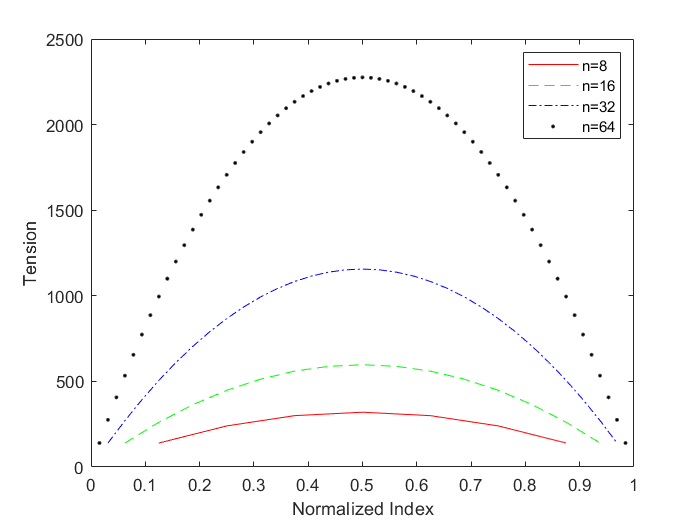
\includegraphics[width=1\linewidth]{Q2a_tension(i).png}
}
\hfill
\subfloat[(ii)]{\label{fig:(ii)}
\centering

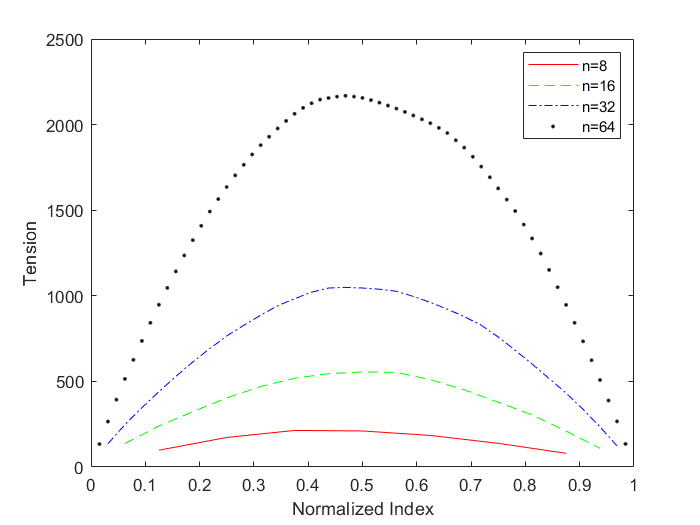
\includegraphics[width=1\linewidth]{Q2a_tension(ii).png}
}

\caption{Tension Vector Components v.s. Normalized Index}
\label{fig:question 2a}
\end{figure}

Here is the log-log plot of the condition number versus n:

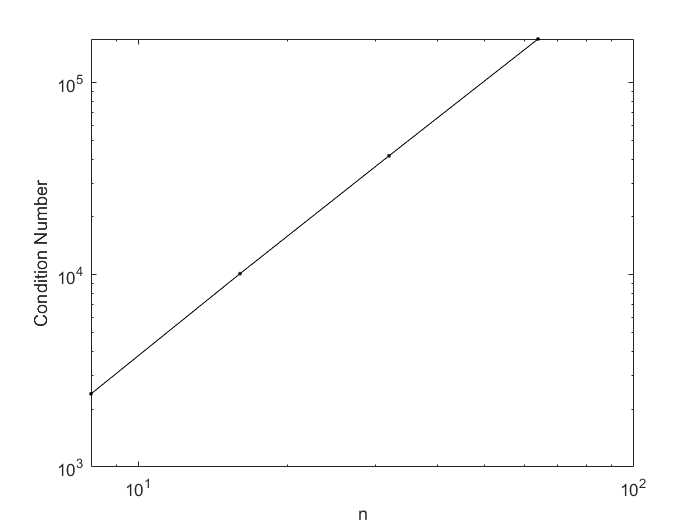
\includegraphics[scale=0.5]{Q2a_loglog.png}

-Comment on how the acceleration and the maximum and minimum tensions behave with n:

N denotes the number of parachutists.

For the trial (i), as n increases, the acceleration and the minimum tension remain constant. The maximum tension, however, is positively correlated with n in a linear manner. the max tension approximately doubles along with a double in n.

For the trial (ii), both of the maximum and minimum tension grow as n increases, but as for the acceleration, it slightly decreases with the growth of n, but in general, it's hard to assure any clear relationship between the minimum tension and n due to the randomness of drag coefficients and mass of parachutists.

-Comment on how the components of the tension vectors vary with their index:

From Figure1: Tension Vector Components v.s. Normalized Index, we can see that for both cases, (i) and (ii), the tension values first increase then decrease with the increasing number of parachutists i.e. n, in an approximately symmetric way. Due to the randomness in (ii), there are some oscillations in values of tension, which affects the symmetry moderately.

-Comment on where (for which i) the max tension occurs:

The maximum tension is attained when the normalized index equals 0.5, so in terms of i, $i = \frac{n}{2}$ for each choice of n, that is, the parachutist right in the middle undertakes the largest tension force.

-Comment on how the condition numbers behave with n:

The numerical results show that in both cases, the condition numbers climb up as n increases and it's interesting to note that fixing n, the condition numbers for (i) and (ii) are very close to each other. Moreover, as n doubles, the value of condition numbers rises fourfold, which indicates a warning for the singularity of our linear system.

In the log-log plot, there is a clear positive and linear relationship between the condition numbers and n, so the slope of this linear function can be interpreted as the n-elasticity of the condition number, that is, the percentage change of the condition number in response to a unit percentage change in n.

Here we illustrate the sparsity patterns of A, P, L, U in a 2x2 format:

\begin{figure}[H]
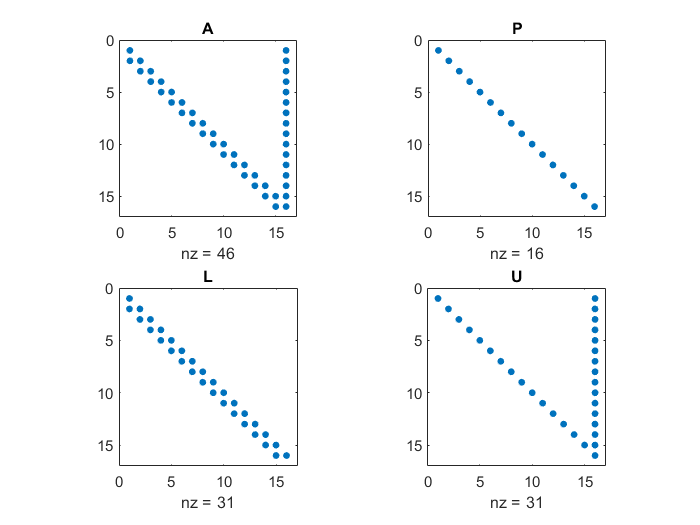
\includegraphics[scale=0.8]{sparsity_pattern.png}
\caption{Plot of Sparsity Patterns}
\end{figure}

Comment: 

The patterns agree with my expectation. The last column of matrix A denotes the mass of n parachutists, which cannot be zero, realistically speaking. Also, for all interior parachutists, they receive two types of tension forces on the opposite direction, which is demonstrated as two non-zero entries in each interior row(excluding entries of the last column).

The followings are the codes I used to output the results:

\begin{lstlisting}
% Q2A (i)
g = 9.81;
v = 6;
ni = [8 16 32 64];
%(i) 
% define containers
t = zeros(64);
cond_num = [0 0 0 0];
for n = ni
    
% construct the matrix A
m1 = linspace(50,100,n)';
c1 = 50 - 20*linspace(0,1,n)';
e=ones(n, 1);
A1=spdiags([-e, e], [-1, 0], n, n); 
A1(:, end) = -m1;

% construct vector b
b1 = c1*v-m1*g;

% solve the system of equations using backslash
t1 = A1\b1;

% condition number of A
kappa1 = condest(A1);

% print the output
fprintf('n: %3d max(t): %10.3e min(t): %10.3e acceleration: %10.3e condition number: %10.3e0\n',...
n, max(t1), min(t1), t1(n), kappa1);

% store the tension value in t for each n
s(1:n,log2(n/8)+1) = t1;

%store the condition number in cond_num for each n
cond_num(log2(n/8)+1) = kappa1;
end

% plot the tension components v.s. normalized index
plot([1:ni(1)-1]/ni(1), s(1:ni(1)-1, 1), 'r-', ...
[1:ni(2)-1]/ni(2), s(1:ni(2)-1, 2), 'g--', ...
[1:ni(3)-1]/ni(3), s(1:ni(3)-1, 3), 'b-.', ...
[1:ni(4)-1]/ni(4), s(1:ni(4)-1, 4), 'k.');
xlabel('Normalized Index');
ylabel('Tension');
legend('n=8','n=16','n=32','n=64');

% plot in log-log scale of kappa v.s. n
loglog(ni,cond_num,'k.-'); 
xlabel('n');
ylabel('Condition Number'); 
%%%%%%%%%%%%%%%%%%%%%%%%%%%%%%%%%%%%%%%%%%%%%%%%%%%%%%%%%
%(ii)
g = 9.81;
v = 6;
t = zeros(64);
ni = [8 16 32 64];
for n = ni
    
% construct the matrix A
m2 = sort(50 + 50*rand(n, 1), 'ascend');
c2=sort(30 + 20*rand(n, 1), 'descend');
e=ones(n, 1);
A2=spdiags([-e, e], [-1, 0], n, n); 
A2(:, end) = -m2;

% construct vector b
b2 = c2*v-m2*g;

% solve the system of equations using backslash
t2 = A2\b2;

% condition number of A
kappa2 = condest(A2);

% print the output
fprintf('n: %3d max(t): %10.3e min(t): %10.3e acceleration: ...
%10.3e condition number: %10.3e0\n',...
n, max(t2), min(t2), t2(n), kappa2);

% store in s
t(1:n,log2(n/8)+1) = t2;
end

% plot the tension components v.s. normalized index
plot([1:ni(1)-1]/ni(1), t(1:ni(1)-1, 1), 'r-', ...
[1:ni(2)-1]/ni(2), t(1:ni(2)-1, 2), 'g--', ...
[1:ni(3)-1]/ni(3), t(1:ni(3)-1, 3), 'b-.', ...
[1:ni(4)-1]/ni(4), t(1:ni(4)-1, 4), 'k.');
xlabel('Normalized Index');
ylabel('Tension');
legend('n=8','n=16','n=32','n=64');
%%%%%%%%%%%%%%%%%%%%%%%%%%%%%%%%%%%%%%%%%%%%%
% sparsity patterns of A, P, L, U when n=16
m16 = linspace(50,100,16)';
c16 = 50 - 20*linspace(0,1,16)';
e16=ones(16, 1);
A16=spdiags([-e, e], [-1, 0], 16, 16); 
A16(:, end) = -m16;
[L16,U16,P16] = lu(A16);

subplot(2,2,1)
spy(A16)
title('A');
subplot(2,2,2)
spy(P16)
title('P');
subplot(2,2,3)
spy(L16)
title('L');
subplot(2,2,4)
spy(U16)
title('U');
\end{lstlisting}

(b)

\[
A = \begin{bmatrix} 
    1 & 0 & \dots & -m_1\\
    -1& 1 & 0 & -m_2\\
    0 &-1 & \ddots  & \vdots\\
    0 &        &  & -m_n
    \end{bmatrix}
\]
Excluding the last column, all diagonal entries are 1 and all sub-diagonal entries are -1. The last column contains all mass information of n parachutists, that is, $a_{kn} = -m_k\ for\ k = 1,2,...n$.

Now we apply LU factorization with row pivoting to A. Notice that for all columns of A except the last column, there are only two non-zero entries with equal absolute values. As a result, at each step of Gauss Elimination, every row stays at their initial position and there's no row interchanges happening.

Each permutation matrix $P_k, k=1,2...n-1$ is the identity matrix $I$, so is the total permutation matrix $P = \Pi_{k=1}^{n-1} I = I^{n-1} = I$.That is, conducting row pivoting or not doesn't affect the final result.

Consider the first step of GE, $\rho_1 = [1\ 0 \ 0 \dots -m_1]$, $\rho_2 = [-1 \ 1 \ 0 \ \dots -m_2 ]$, then do the row operation $\rho_2^{(1)}  = \rho_2 - (-1)\rho_1 = [0\ 1\ 0\ \dots -(m_1+m_2)]$, eliminating the entry in the first column to 0. Since the $a_{p1}$ entries of the remaining rows($p>2$) are already zeros, $\rho_p^{(1)}  = \rho_p - (0)\rho_1 = [0\ \dots \ -1 \ 1 \ \dots \ -(m_1+m_p)]$. Therefore, the first column of factor L is $[1\ -1\ 0 \dots 0]'$ and the second row of factor U is $[0\ 1\ 0\ \dots \ -(m_1+m_2)]$.

In general, at the kth step of GE, we only have 1 row operation that make changes, $\rho^{(k)}_{k+1} = \rho_{k+1}^{(k-1)}-(-1)\rho_{k}^{(k-1)}$ and other rows remaining the same i.e. $\rho_p^{(k)}  = \rho_p^{(k-1)} - (0)\rho_{k}^{(k-1)} = \rho_p^{(k-1)}$.

After all steps of GE, we will get factors L and U of the following form
\[
L = \begin{bmatrix} 
     1& 0 & \dots & 0 & 0\\
    -1& 1 & 0 & \dots & 0\\
     0&-1 & 1&      &  0\\
\vdots& \vdots &-1& \ddots & \vdots\\
     0& 0 & \dots & -1 & 1
    \end{bmatrix}
\]
L is lower bi-diagonal with all 1's on the diagonal and -1's on the sub-diagonal, and 
\[
U = \begin{bmatrix} 
     1& 0 & \dots & 0 & -m_1\\
     0& 1 & 0 & \dots & -(m_1+m_2)\\
     0& 0 & 1&      &  -\sum_{k = 1}^3 m_k\\
\vdots& \vdots & 0 & \ddots & \vdots\\
     0& 0 & \dots & 0 & -\sum_{k = 1}^n m_k
    \end{bmatrix}
\]
U has all 1's on the diagonal and all entries of the last column in the form $a_{pn} = -\sum_{k=1}^p m_k$, the summation of all previous entries in the last column.

Notice that the forms of L, U and P are exactly what we saw from the plot of sparsity patterns in part (a).

(c)

Now we would like to solve $At = Pb = b \Rightarrow LUt_n = c_n v-m_n g$.

Denote $Ut_n = y_n$, we first solve $Ly_n = c_n v-m_n g$. By forward substitution, 
\begin{equation}
\begin{aligned}
y_1 &= c_1 v - m_1 g\\
-y_1 + y_2 = c_2 v - m_2 g \Rightarrow y_2 &= (c_1+c_2)v-(m_1+m_2)g\\
...\\
y_p &= (\sum_{k = 1}^p c_k)v - (\sum_{k = 1}^p m_k)g\\
...\\
y_n &= (\sum_{k = 1}^n c_k)v - (\sum_{k = 1}^n m_k)g
\nonumber
\end{aligned}
\end{equation}

Then apply backward substitution to solve $Ut_n = y_n$, we can first get the acceleration $a = t_n$
\begin{equation}
\begin{aligned}
-\sum_{k = 1}^n m_k t_n &= y_n\\
t_n &= \frac{(\sum_{k = 1}^n c_k)v - (\sum_{k = 1}^n m_k)g}{-\sum_{k = 1}^n m_k}\\
a &= g - \frac{(\sum_{k = 1}^n c_k)v}{\sum_{k = 1}^n m_k}
\nonumber
\end{aligned}
\end{equation}

then for the tension forces,
\begin{equation}
\begin{aligned}
t_{n-1} &= y_{n-1}+ a\sum_{k = 1}^{n-1}m_k \\
t_{n-1} &= (\sum_{k = 1}^{n-1}c_k) v-\frac{\sum_{k = 1}^{n-1}m_k}{\sum_{k = 1}^{n}m_k}\sum_{k = 1}^{n}c_k v
\nonumber
\end{aligned}
\end{equation}

In general, $t_p = y_{n-p} + \sum_{k=1}^{n-2}m_k t_{n-p+1}$.

\section{Question 3}

(a)

The output of the experiment:\\
n:  2 condition number:  1.93e+01 relative error:  6.66e-16 norm of residual:  0.00e+00 norm of b_n:  2.32e+00\\
n:  3 condition number:  5.24e+02 relative error:  1.07e-14 norm of residual:  0.00e+00 norm of b_n:  3.84e+00\\
n:  4 condition number:  1.55e+04 relative error:  1.21e-13 norm of residual:  0.00e+00 norm of b_n:  5.55e+00\\
n:  5 condition number:  4.77e+05 relative error:  5.25e-12 norm of residual:  4.44e-16 norm of b_n:  7.42e+00\\
n:  6 condition number:  1.50e+07 relative error:  4.73e-11 norm of residual:  6.28e-16 norm of b_n:  9.46e+00\\
n:  7 condition number:  4.75e+08 relative error:  9.31e-09 norm of residual:  7.69e-16 norm of b_n:  1.16e+01\\
n:  8 condition number:  1.53e+10 relative error:  1.44e-07 norm of residual:  1.40e-15 norm of b_n:  1.40e+01\\
n:  9 condition number:  4.93e+11 relative error:  7.38e-06 norm of residual:  2.43e-15 norm of b_n:  1.64e+01\\
n: 10 condition number:  1.60e+13 relative error:  1.66e-04 norm of residual:  9.93e-16 norm of b_n:  1.90e+01\\
n: 11 condition number:  5.22e+14 relative error:  1.43e-03 norm of residual:  2.95e-15 norm of b_n:  2.17e+01\\
Warning: Matrix is close to singular or badly scaled. Results may be inaccurate. RCOND =  2.684500e-17. \\
> In Q3 (line 16)\\
 
n: 12 condition number:  1.62e+16 relative error:  9.25e-02 norm of residual:  2.66e-15 norm of b_n:  2.45e+01\\
Warning: Matrix is close to singular or badly scaled. Results may be inaccurate. RCOND =  3.330077e-18. \\
> In Q3 (line 16)\\
 
n: 13 condition number:  4.79e+17 relative error:  1.55e-01 norm of residual:  2.18e-15 norm of b_n:  2.74e+01\\

MATLAB gave a warning saying that \textbf{'Warning: Matrix is close to singular or badly scaled. Results may be inaccurate.'}. Such warnings appear as n>10, which confirm the given fact that the Hilbert matrices are very ill-conditioned once n increases beyond a certain value. In our case, such value equals 10.

As the order of the Hilbert matrix $H_n$ increases, the condition numbers rocket up exponentially. The norm of residuals remain to be constantly small but the computational relative error keeps increasing along with the growth of n.

Such large condition numbers indicate a large uncertainty in the solution of the system of equations $H_n x_n=b_n$. Larger the condition number, more ill-conditioned the matrix is, and closer the corresponding linear system is to singularity.

Moreover, with large condition numbers, even though the residuals continue to be relatively small, it is false to imply that the relative errors are also small.

(b)

The semilogy-scale plot of the condition number, $e(\frac{||x_n-\hat{x_n}||}{|x_n|})$ and $\frac{c(n)r(n)}{v(n)}$ versus n is shown below:

\begin{figure}[H]
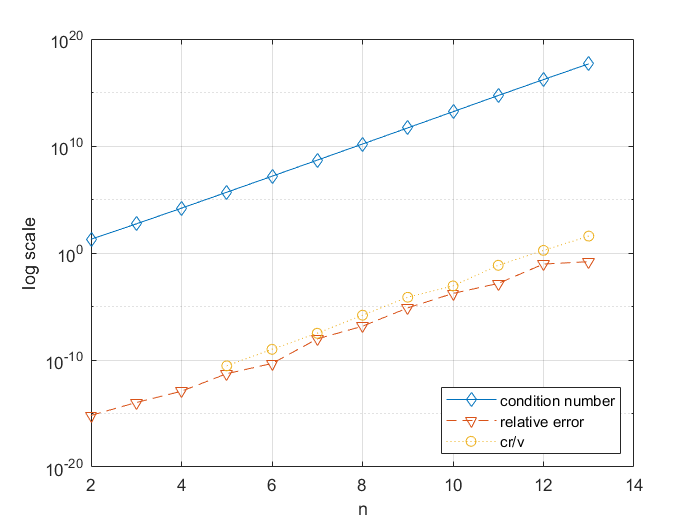
\includegraphics[scale=0.8]{Q3.png}
\caption{Semilogy-scale plot}
\end{figure}

As we can see from the plot, all 3 metrics are increasing as the matrix order n increases. The expression $c(n)r(n)}{v(n)} = \kappa_n \frac{r_n}{b_n}$ where $r_n$ denotes the residual corresponding to the computed solution and $b_n$ denotes the right side vector of the equation $H_n x_n = b_n$. Therefore, this expression is an upper bound for the relative error $\frac{||e_n||}{||x_n||} = \frac{||x_n-\hat{x_n}||}{||x_n||}$ and this upper bound is also increasing with n.

In summary, all of these 3 metrics agree with the numerical computations we derive from part (a) as well as the theory.

The followings are the codes I used for question 3:
\begin{lstlisting}
% (a)

ni = [2:13];
c = zeros(1,13);
e = zeros(1,13);
r = zeros(1,13);
v = zeros(1,13); % some containers
for n = ni
    Hn = hilb(n);
    bn = zeros(1,n)';
    for i =[1:n]
        syms j
        bni = symsum(j/(i+j-1),j,1,n);
        bn(i) = bni;
    end
    xn_hat = Hn\bn; % where warnings happen
    xn = [1:n]';
    rn = bn - Hn*xn_hat;
    kappan = cond(Hn);
    rel_error = norm(xn-xn_hat)/norm(xn);
    norm_rn = norm(rn);
    norm_bn = norm(bn);
    c(n) = kappan;
    e(n) = rel_error;
    r(n) = norm_rn;
    v(n) = norm_bn;
    fprintf('n: %2d condition number: %9.2e relative error:...
    %9.2e norm of residual: 9.2e norm of b_n: %9.2e\n', ...
        n, kappan, rel_error, norm_rn, norm_bn);
end
%%%%%%%%%%%%%%%%%%%%%%%%%%%%%%%%%%%%%%%%%%

%(b)
c = c([2:end]);
e = e([2:end]);
r = r([2:end]);
v = v([2:end]);
semilogy(ni,c,'-d',ni,e,'--v',ni,c.*r./v,':o')
hold on
grid on
xlabel('n')
ylabel('log scale')
legend('condition number', 'relative error','cr/v','Location','southeast');
\end{lstlisting}
\end{document}
